\section{Evaluation}
\label{Sec:Evaluation}

	\subsection{Goals and Research Questions}
	\label{Sec:Goals}
	In order to evaluate how effective is our tool in assisting the developers, we empirically evaluated our tool as well as conducted an a user study. We wish to answer the following research questions in our study.
	\begin{description}
		\item[RQ1:] What is the convergence rate for number of unique CSS selectors verses number of DOM states?
		\item[RQ2:] How accurate are the code-completion suggestions provided by the tool?
		\item[RQ3:] What is the time overhead cost incurred by the tool?
		\item[RQ4:] Does \dompletion make programming tasks faster without compromising correctness of the program?
		\item[RQ5:] Does \dompletion make debugging tasks easier?
	\end{description}
	
	\subsection{Methodology}
	\label{Sec:Methodology}
	The subsections that follow address each of the above questions. We used a php-\javascript based web application Phormer\footnote{\url{http://p.horm.org/er/}} as a case study to evaluate our tool. An overview of the evaluation methodology we have used to answer each research questions is shown below.
	
	\headbf{RQ1 Approach} To answer this question, we crawled the web application in a random order until the number of minimized css selectors become constant. We also conducted this study on 5 major websites including a few listed in top 100 websites on Alexa\footnote{\url{http://www.alexa.com/topsites}}.  We then reported the number of total, unique and minimized \css selectors for each website.
	
	\headbf{RQ2: Approach} To answer this question, we used our tool to generate suggestions for the existing \javascript code in the selected web application. We then manually match the list of generated suggestions to the existing text within the \javascript code. The list of generated suggestions is considered valid if one of the suggestions matches the \css selector used within the code where the code completion was initiated. 
		
	\headbf{RQ3: Approach} To answer this question, we used our tool to generate suggestions for the selected web application as in RQ2. We then report the time taken by the tool to generate these suggestions. We also report the time taken by the tool in the initialization phase.
		
	\headbf{RQ4: Approach} To answer this question, we conducted a user study where users were asked to write \javascript code, that interacts with the DOM to complete certain tasks for the same web application. We compared the time taken by users to complete he task with and without our tool.
	
	\headbf{RQ5: Approach} To answer this question, we conducted a study similar to previous question. We injected bugs (DOM related) in the \javascript code and asked the users to find out these bugs. We compared the time taken by the users to complete the task with and without our tool.
	 	
	\begin{figure}
		\centering
		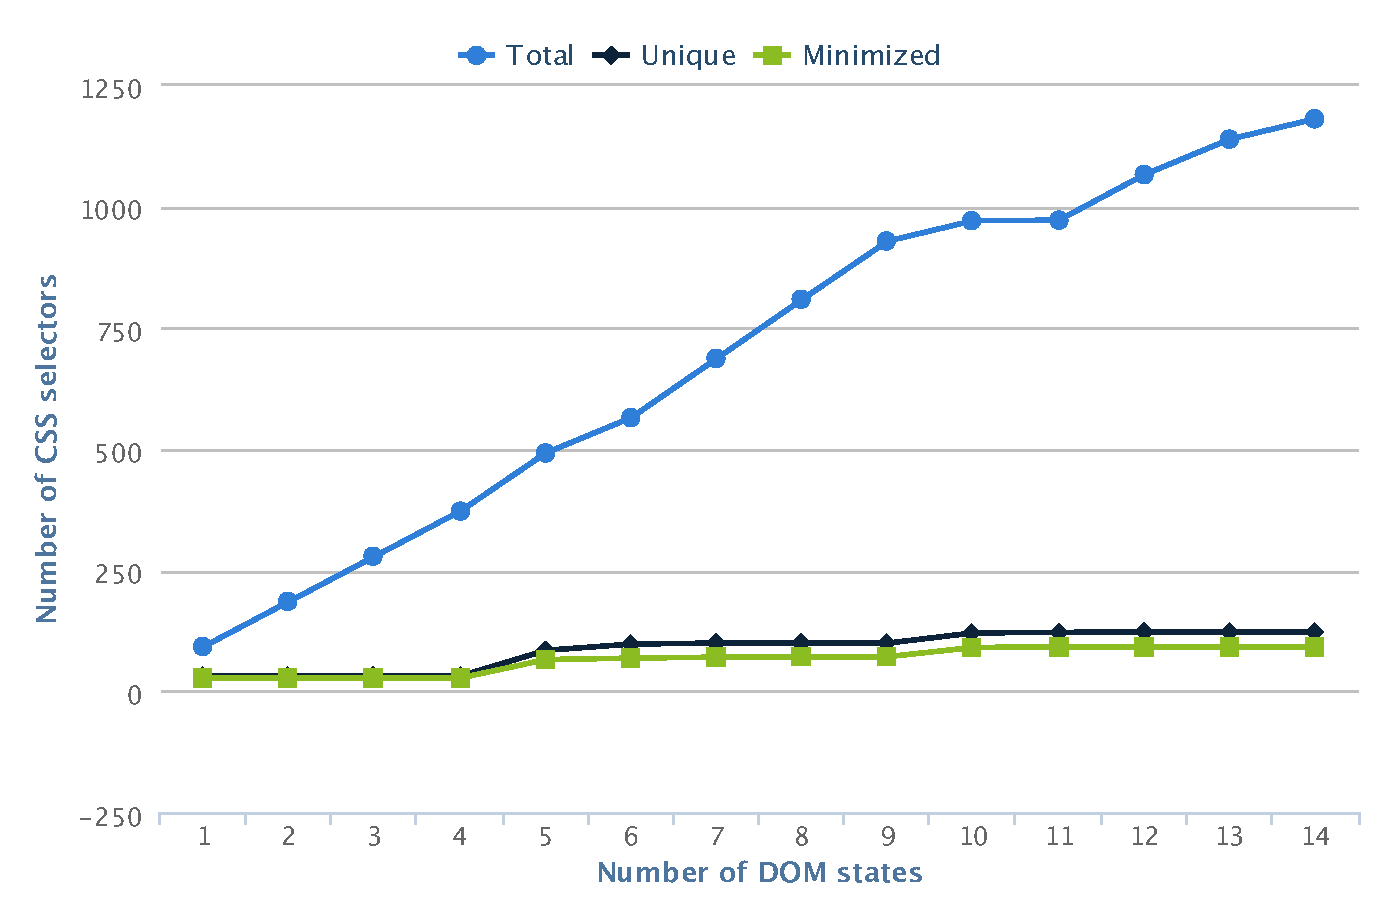
\includegraphics[width=85mm]{images/phormer.pdf}
		\caption{CSS Selectors for Phormer Web Application}
		\label{Fig:Phormer}
	\end{figure}
	
	\begin{figure}
		\centering
		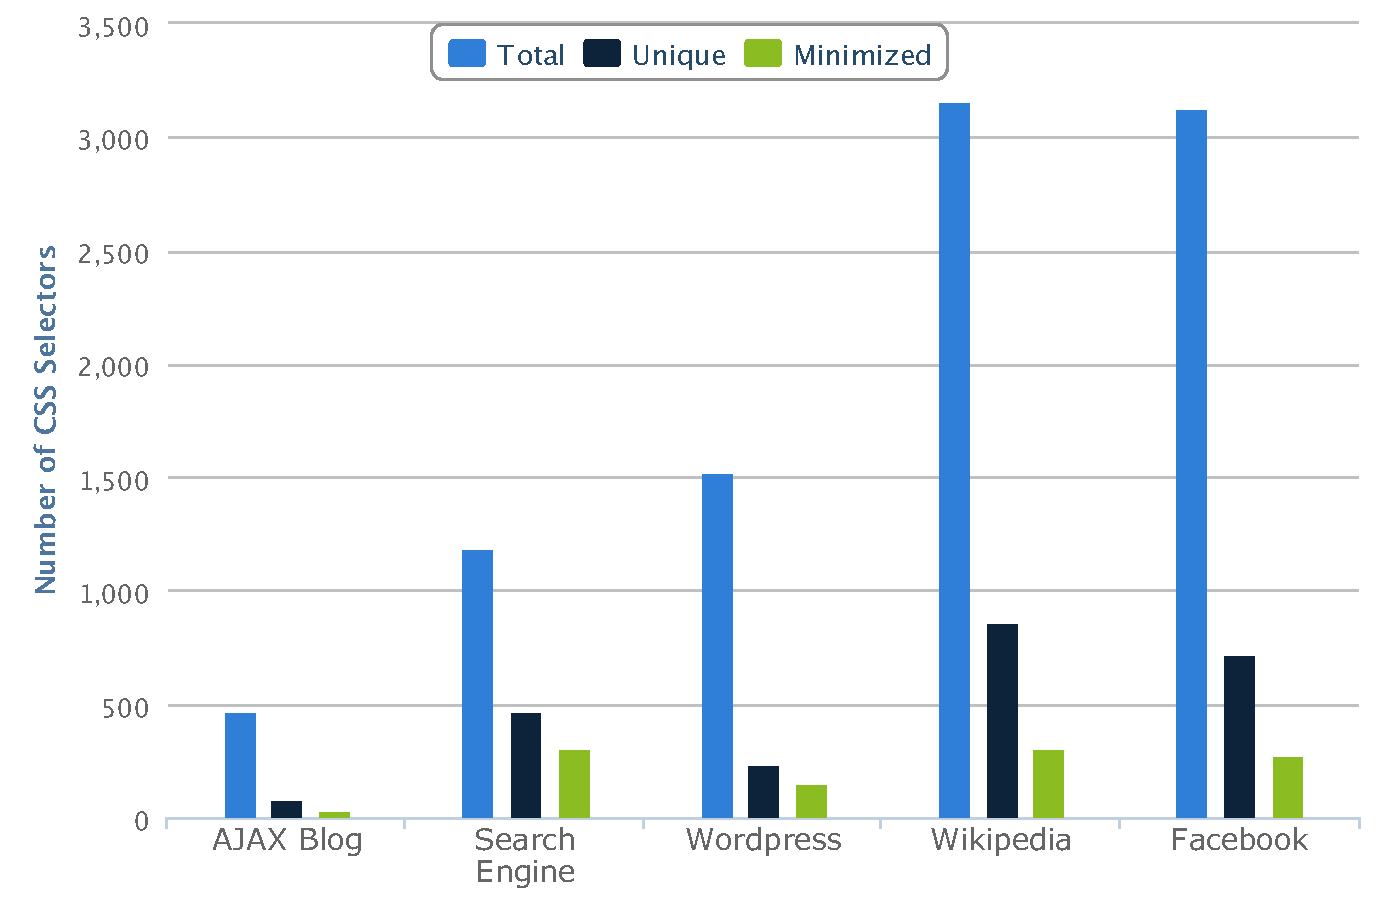
\includegraphics[width=85mm]{images/convergence.pdf}
		\caption{Convergence of \css selectors for different websites}
		\label{Fig:Convergence}
	\end{figure}
		
	\subsection{Convergence rate for \css selectors}
	\label{Sec:Convergence}
	To answer RQ1, we crawled the web application starting with the home page. We counted the total number of \css selectors, unique \css selectors and minimized \css selectors. For every successive DOM states we included the list of \css selectors from the previous states, therefore only measuring the new \css selectors encountered at each state. We also crawled 5 web applications, few among them were listed in top 100 websites on Alexa: Facebook\footnote{\url{https://www.facebook.com/}} (User specific content), Wikipedia\footnote{\url{https://www.wikipedia.org/}} (User generated content), Bing\footnote{\url{http://www.bing.com/}} (Search Engine), Wordpress Blog\footnote{\url{http://blogs.ubc.ca/karthik/}} and AJAX based blog\footnote{\url{http://www.ece.ubc.ca/~amesbah/}}. All the applications chosen for analysis were dynamic in nature, \ie the DOM tree generated for these websites is either user or input dependent. Two of the analyzed were blogs, where content of DOM tree is dependent on one single user (blog admin) and similar for other user. 

	\figref{Phormer} represent the results at the  end of analysis of each DOM state for the Phormer web application. As seen from the graph, the total number of \css selectors increase linearly with each DOM state whereas total number of minimized \css selectors tend to become constant with the growing number of DOM states. \figref{Convergence} represent the result of analysis for the other websites. These websites were crawled until the total number of minimized \css selectors tend to become constant as in the previous case. We then report the accumulated number of \css selectors for each website.
	
	As seen from the results, all of the above mentioned websites exhibit patterns in their \css selectors and these patterns tend to converge quickly. The patterns once detected can be used to predict the structure of DOM states that were not encountered during the crawling phase. Therefore, the code-completion system can detect patterns and provide suggestions even for the unseen but similar DOM states.
	
	\finding{DOM states for a particular website exhibit patters in their \css selectors and these patterns tend to converge with increasing number of DOM states. \label{Finding:Convergence}}
	
	
	\begin{figure}
		\centering
		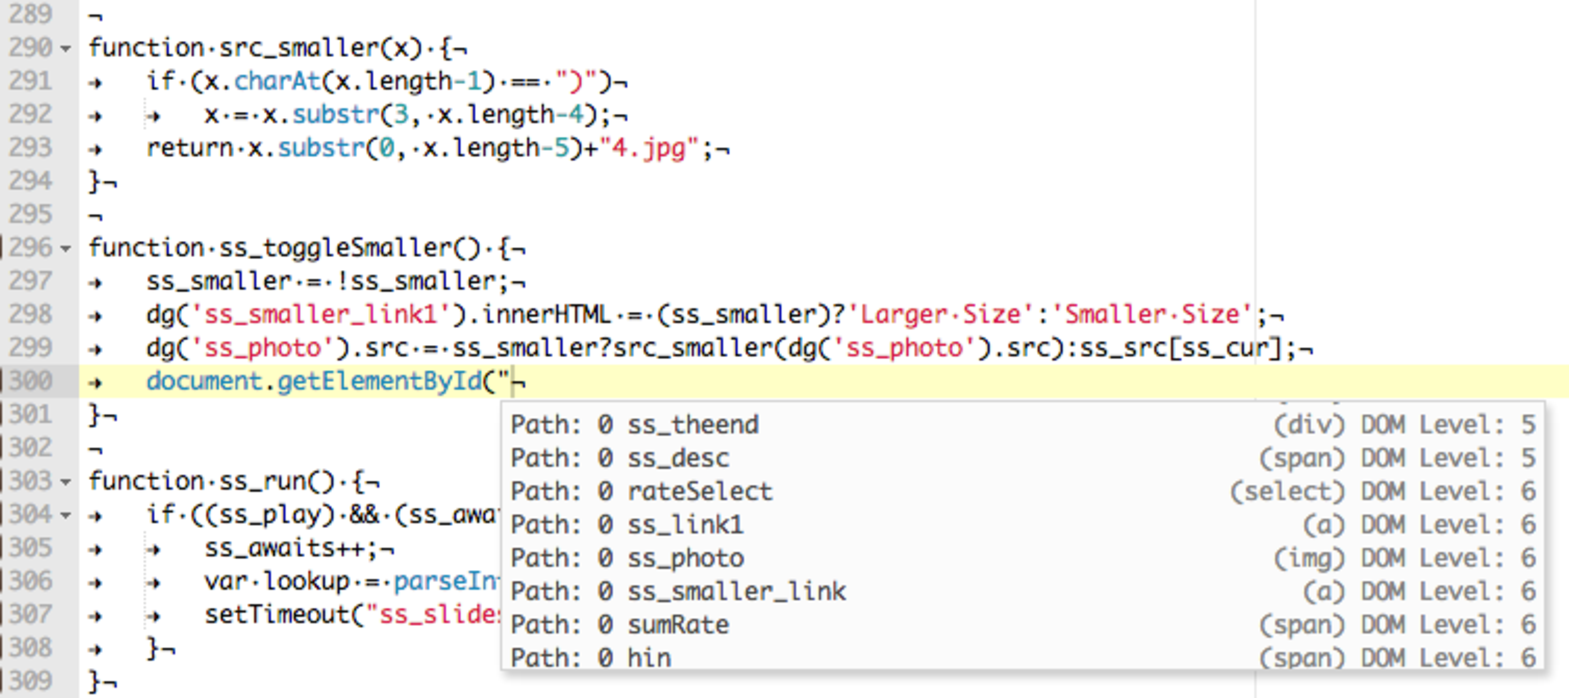
\includegraphics[width=85mm]{images/accuracy.pdf}
		\caption{Code completion suggestions generated using \dompletion}
		\label{Fig:Accuracy}
	\end{figure}
	
	\begin{table}
	{
		\scriptsize
		\begin{tabular}{ p{3.8cm} | p{3.8cm}}
  			\hline                        
  			\textbf{Output} & \textbf{No. of use cases} \\ \hline \hline
  			Valid Suggestions &  40 \\ \hline
			Invalid Suggestions & 7 \\ \hline
			Error & 6 \\ \hline
			Total & 53 \\ 
			\hline  
		\end{tabular}
	}
	\caption {\dompletion evaluation}
	\label{Table:Accuracy}		
	\end{table}
	
	
	
	
	\subsection{Accuracy of \dompletion}
	\label{Sec:Accuracy}
	To answer RQ2, we utilized our tool to perform code-completion for every DOM interaction within the \javascript code and analyzed if the suggestions provided by the tool are valid or not. A list of suggestions is considered valid if one of those suggestions represent the actual keyword used within the code.
	
	In total, there were 53 calls to the \texttt{getElementById} function within the \javascript code. We performed code-completion using our tool for these calls.    \figref{Accuracy} represents the valid output where the list of suggestions contain the ID that was used within the code. We used the code-completion tool to generate suggestions at Line 300, and see if the element ID used at Line 299 is available in the suggestions. 
	
	\tabref{Accuracy} represents the results of our analysis. Invalid suggestions represent the case, when our tool did not provide the required element as a suggestion. This was due to insufficient crawling of the website, which can be overcome by providing information like login ids and password to crawl the application extensively. The error represents the case when our tool failed to analyze the \javascript code. This was due to improper handling of parameters, un-handled \texttt{http} requests, alert boxes, etc. However, these are just implementation issues and we plan to improve upon them in the next version of our tool. As seen from the results, \dompletion can provide code completion suggestions with high accuracy of about 75\% of all cases and with an accuracy of about 87\% if the DOM states are crawled extensively \ie excluding the invalid suggestions case.
	
	\finding{\dompletion can provide code-completion suggestions with an accuracy of about 87\% . \label{Finding:Accuracy}}
	
	
	\subsection{Time Overhead by \dompletion}
	\label{SecOverhead}
	To answer RQ3, \ie time overhead we report the time take to crawl the web application when initializing the tool and the time take to generate code-completion suggestions when the programmer activates the code-completion menu.
	
		\begin{table}
	{
		\scriptsize
		\begin{tabular}{ p{3.8cm} | p{3.8cm}}
  			\hline                        
  			\textbf{No. of DOM states crawled} & \textbf{Total time taken (in Seconds)} \\ \hline \hline
  			1 & 18  \\ \hline
			2 & 23 \\ \hline
			3 & 27  \\ \hline
			4 & 34  \\ \hline
			5 & 43  \\ \hline
			6 & 56  \\ \hline
			7 & 57  \\ \hline
			8 & 66  \\ \hline
			9 & 83  \\ \hline
			10 & 94  \\ \hline
			11 & 117  \\ \hline
			12 & 148  \\ \hline
			13 & 157  \\ \hline
			14 & 173  \\ \hline
			\hline  
		\end{tabular}
	}
	\caption {Time overhead incurred during DOM Analysis phase}
	\label{Table:Time}		
	\end{table}
	\headbf{DOM Analysis}
	When the \dompletion tool is initialized it first needs to gather data about the possible DOM states of the web application. This data is then used to provide code-completion suggestions to the developers. Once the tool is initialized, the crawling phase still continues in the background. However, we do not consider time over head for that as it in done in background and unnoticed by the developer. Time required to analyze the DOM state depends upon the size of DOM tree. Larger the DOM tree, more time it takes to analyze the DOM state.
	
	\tabref{Time} represent the results of our analysis and the time taken to crawl each DOM state. For each DOM state we report the total time consumed till then \ie for DOM state 10, we report the time taken to crawl DOM states 1 to 10. As shown in the table, it takes around 173 seconds to crawl 14 DOM states \ie crawl until number of minimized \css selector tend to become constant for the particular web application (\secref{Convergence}). Even though the time taken to analyze the DOM states is not negligible, the overhead is just incurred once. 
	
	\headbf{Code Analysis}
	The code-completion phase starts when the developer activates the tool by pressing \texttt{cntrl} + \texttt{space} keys or any other combination set by the developer to activate the code-completion module. The time required to analyze the code can vary depending upon the number of conditional statements within the code, size of code that needs to be analyzed and number of functions defined within the code. We calculated the time for different code-completion tasks in the given \javascript code. The time required to analyze the code vary from 2 to 8 seconds.
	
	\finding{\dompletion can provide code-completion suggestions within minimal time overhead ranging between 2 to 8 seconds.} 
	
